\documentclass{article}
\usepackage{../verslagstyle}



\begin{document}
	\title{Labo 2}
	\author{Bert De Saffel}
	\date{19 februari 2019}
	\maketitle
	
	\section{Oplosmethode}
	De gebruikte programmeertaal is Python. Elke oefening is een apart bestand \texttt{labo2\_ex$[2-7]$.py}. Om de afbeeldingen te vergelijken wordt er gekozen om de functie \textbf{hconcat} (uitleg in sectie 2) te gebruiken. Op die manier kunnen er meerdere images in dezelfde window getoond worden. De aangepaste figuren worden wel nog apart opgeslagen onder de vorm \texttt{[bestandsnaam]EX[oefeningnummer].png}.
	
	\section{Gebruikte functies}
	\begin{itemize}
		 \item \textbf{GuassianBlur(src, ksize, sigmaX[, dst[, sigmaY[, borderType]]]) $\rightarrow$ dst}
		 
		 Deze functie is in staat om een figuur te vervagen volgens een twee-dimensionale normaalverdeling. Het \textit{ksize} attribuut is een paar van getallen die de dimensies van de zogenaamde kernel, een matrix met gewichten, bevat. De gewichten worden gekozen aan de hand van de twee-dimensionale normaalverdeling rond de middelste pixel, en wordt voorgesteld door volgende functie:
		 $$G(x, y) = \frac{1}{2\pi\sigma^2}e^{-\frac{x^2 + y^2}{2\sigma^2}}$$
		 
		 Elke pixel wordt dan vervangen door het gewogen gemiddelde van zijn naburige pixels. Tot slot moet ook nog $\sigma$ gedefinieerd worden. OpenCV laat toe om enkel \textit{sigmaX} in te vullen. Een lege \textit{sigmaY} krijgt dezelfde waarde als \textit{sigmaX}, maar kan natuurlijk altijd zelf gekozen worden. De variabele $\sigma$ bepaalt de mate in hoeveel er vervaagt wordt, waarbij een grotere waarde meer vervaagt. Het onderscheid tussen \textit{sigmaX} en \textit{sigmaY} is dan respectievelijk de vervaging in de X-richting en de Y-richting.
		
		 \item \textbf{medianBlur(src, ksize[, dst]) $\rightarrow$ dst}
		 
		 Deze functie vervaagt ook een figuur zoals guassianBlur, maar met het verschil dat de waarde van de pixels niet vervangen worden door het gewogen gemiddelde van de naburige pixels, maar door de mediaan van de naburige pixels. Ook is hier is de functie van het \textit{ksize} attribuut het aanmaken van een kernel met opgegeven grootte. Het \textit{ksize} attribuut is hier wel geen paar van getallen, maar slechts één oneven getal en bovendien moet deze groter zijn dan 1.
		 
		 \item \textbf{Sobel(src, ddepth, dx, dy[, dst[, ksize[, scale[, delta[, borderType]]]]]) $\rightarrow$ dst}
		 
		 Deze functie is in staat om de eerste, tweede en derde orde afgeleiden te bereken van een figuur. In het labo is enkel de eerste orde afgeleide nodig. De eerste orde afgeleide is in staat om randen van objecten in een figuur te detecteren. Naargelang dat $dx = 1$ of $dy = 1$ zal de functie respectievelijk verticale of horizontale randen detecteren. Voor horizontale randen wordt de volgende matrix gebruikt:
		 
		 $$G_x = \begin{bmatrix}
		 -1 & 0 & +1 \\
		 -2 & 0 & +2 \\
		 -1 & 0 & +1 
		 \end{bmatrix}$$
		 
		 De middelste rij krijgt meer gewicht dan de rij erboven of eronder om de detail van die specifieke rij niet te verliezen. De figuur wordt ook eerst geconverteerd naar een grijsschaal figuur om de complexiteit van de figuur te verminderen. 
		 
		 \item \textbf{filter2D(src, ddepth, kernel[, dst[, anchor[, delta[, borderType]]]]) $\rightarrow$ dst}
		 
		 Deze functie laat toe om een eigen filter te maken. Het \textit{kernel} argument is een eigen gedefinieerde kernel. Het \textit{anchor} attribuut definieert het ankerpunt van de filter. Een waarde van (-1, -1) neemt het centrum als ankerpunt. Voor het labo moet (14, 14) genomen worden. De \textit{delta} parameter laat toe om een optionele waarde toe te voegen aan de gefilterde pixels.
		 
		 \item \textbf{hconcat(src[, dst]) $\rightarrow$ dst}
		 
		 Dit is een handige functie om meerdere images in dezelfde window te tonen. Dit werkt aangezien images eigenlijk matrices zijn, die dus horizontaal of verticaal aan elkaar kunnen geplakt worden. In het geval van hconcat is dit horizontaal. De \textit{src} parameter is een lijst van figuren.
		
		 \item \textbf{absdiff(src1, src2[, dst] $\rightarrow$ dst)} en \textbf{add(src1, src2[, dst[, mask[, dtype]]]) $\rightarrow$ dst}
		 
		 Deze functies laten bewerkingen toe op figuren zoals aftrekken en optellen. Aangezien figuren voorgesteld worden als matrices komt dit neer op bewerkingen op matrices.
		
		
	\end{itemize}
\newpage
	\section{Invoer en uitvoer}

	\subsection*{Opgave 2}
	\begin{figure}[!htb]
		\begin{minipage}{0.48\textwidth}
			\centering
			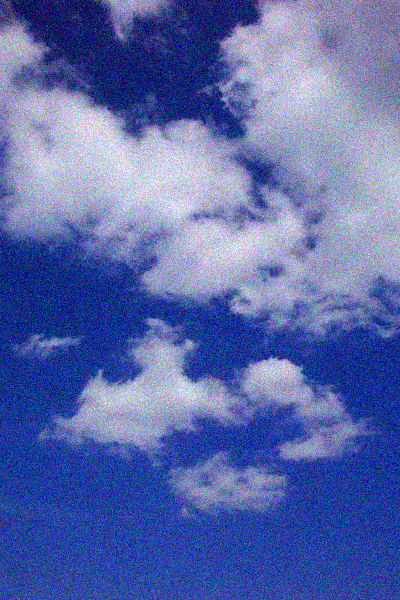
\includegraphics[width=0.9\linewidth]{whitenoise}
			\caption*{}
			\label{Fig:ex2_1}
		\end{minipage}\hfill
		\begin{minipage}{0.48\textwidth}
			\centering
			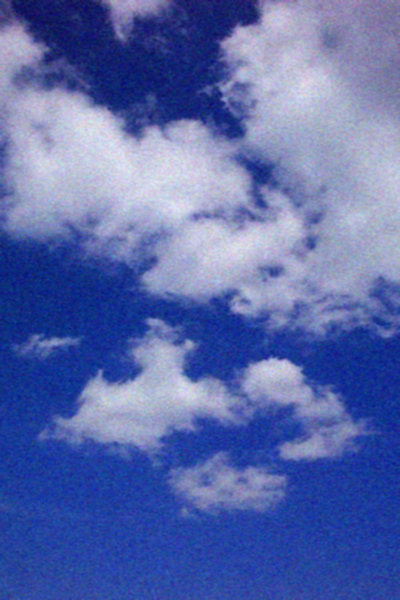
\includegraphics[width=0.9\linewidth]{whitenoiseEX2}
			\caption*{}
			\label{Fig:ex2_2}
		\end{minipage}
	\end{figure}
	\subsection*{Opgave 3}
	
	\begin{figure}[!htb]
		\begin{minipage}{0.48\textwidth}
			\centering
			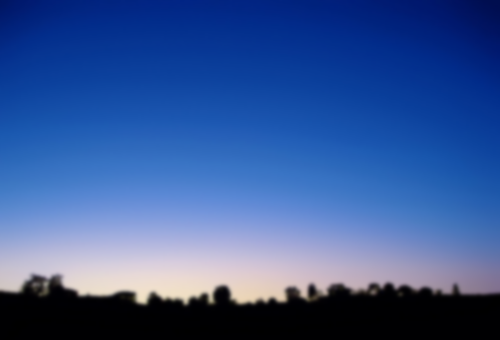
\includegraphics[width=0.9\linewidth]{unsharp}
			\caption*{}
			\label{Fig:ex2_1}
		\end{minipage}\hfill
		\begin{minipage}{0.48\textwidth}
			\centering
			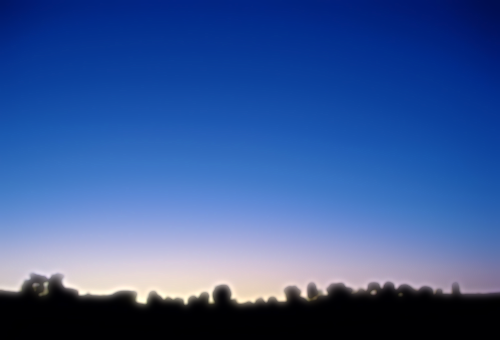
\includegraphics[width=0.9\linewidth]{unsharpEX3}
			\caption*{}
			\label{Fig:ex2_2}
		\end{minipage}
	\end{figure}
\newpage
	\subsection*{Opgave 4}
	\begin{figure}[!htb]
		\begin{minipage}{0.48\textwidth}
			\centering
			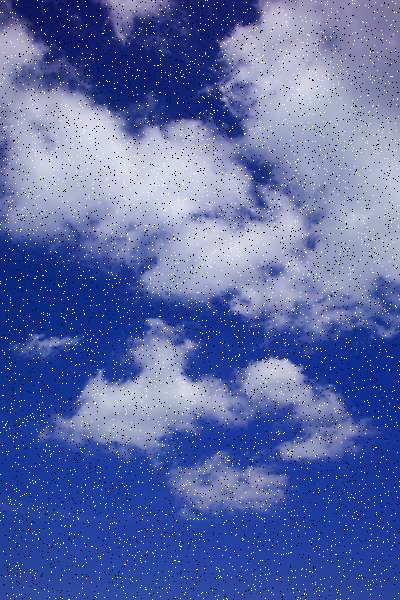
\includegraphics[width=0.9\linewidth]{saltandpeppernoise}
			\caption*{}
			\label{Fig:ex2_1}
		\end{minipage}\hfill
		\begin{minipage}{0.48\textwidth}
			\centering
			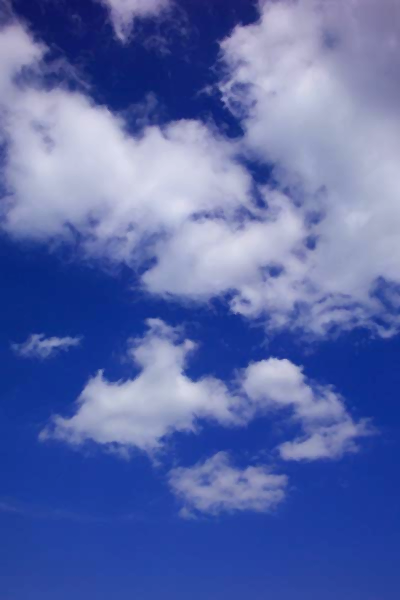
\includegraphics[width=0.9\linewidth]{saltandpeppernoiseEX4}
			\caption*{}
			\label{Fig:ex2_2}
		\end{minipage}
	\end{figure}
	\subsection*{Opgave 5}
	\begin{figure}[!htb]
		\begin{minipage}{0.48\textwidth}
			\centering
			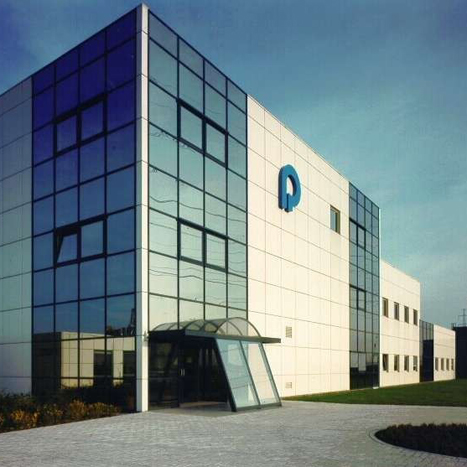
\includegraphics[width=0.9\linewidth]{building}
			\caption*{}
			\label{Fig:ex2_1}
		\end{minipage}\hfill
		\begin{minipage}{0.48\textwidth}
			\centering
			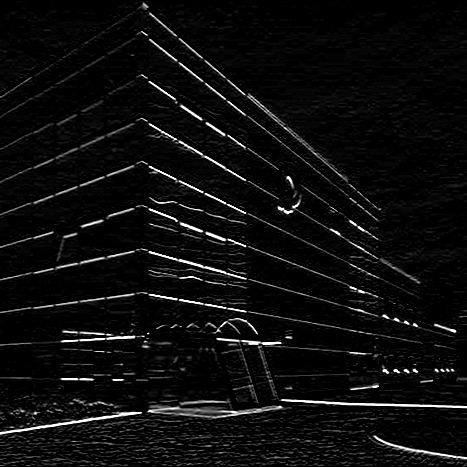
\includegraphics[width=0.9\linewidth]{buildingEX5}
			\caption*{}
			\label{Fig:ex2_2}
		\end{minipage}
	\end{figure}
\newpage
	\subsection*{Opgave 6}
	\begin{figure}[!htb]
		\begin{minipage}{0.48\textwidth}
			\centering
			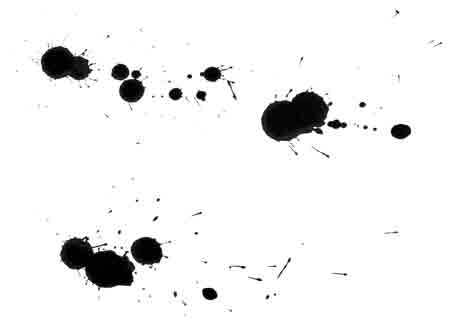
\includegraphics[width=0.9\linewidth]{blots}
			\caption*{}
			\label{Fig:ex2_1}
		\end{minipage}\hfill
		\begin{minipage}{0.48\textwidth}
			\centering
			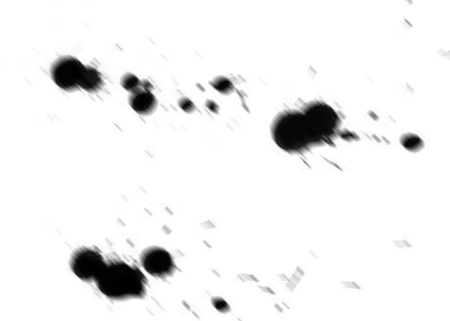
\includegraphics[width=0.9\linewidth]{blotsEX6}
			\caption*{}
			\label{Fig:ex2_2}
		\end{minipage}
	\end{figure}
	
\end{document}